% !TeX TXS-program:compile = txs:///pdflatex/[--shell-escape]
\documentclass[../../../00.FullDoc/tex/ThesisSkeleton-draft2]{subfiles}

%\documentclass[12pt,a4paper,notitlepage,
%draft,
%bibliography=totoc,
%numbers=endperiod,
%appendixprefix=true,
%usenames,dvipsnames]{scrartcl} 
%\usepackage[autooneside=false, draft=false]{scrlayer-scrpage}
%\usepackage{ifdraft} %allows commands dependent on draft status
%\usepackage{scrhack}
%\usepackage{kpfonts}
%\usepackage[dvipsnames]{xcolor} %general colours
%\usepackage{colortbl} % colour for excel tables
%\usepackage{hyperref}
%\usepackage[inline]{enumitem} %inline/horizontal lists
%\hypersetup{
%	draft=true,
%	final=true,
%	colorlinks=true,
%	linktoc=all,
%	linkcolor=MidnightBlue,
%	citecolor=blue
%	%	allcolors=black
%}
%\usepackage{mwe}
%\usepackage{tipa} %IPA
%\usepackage{phonrule} %phonological rules
%\usepackage{amsmath}
%\usepackage{amsfonts}
%\usepackage{soul}
%\usepackage{amssymb}
%\usepackage{graphicx} %insert graphics, pdf etc.
%\usepackage{caption}
%\usepackage{setspace}
%\usepackage{nameref}
%\usepackage{pdfpages}
%\usepackage{csvsimple}
%\usepackage{booktabs, multicol, multirow}
%\usepackage{array}
%\usepackage{float} % float 
%\usepackage[section]{placeins}
%\usepackage{array}
%\usepackage[section]{placeins}
%\usepackage[round]{natbib} %citation package
%\bibliographystyle{agsm}
%\renewcommand{\harvardurl}{\textbf{URL:} \url}
%\usepackage{scrlayer-scrpage}
%\usepackage{blindtext}% dummy text
%\usepackage{subfiles} %subfile functionality
%\usepackage{csvsimple} %import csv tables
%\usepackage{pdflscape} %allow landscape pages
%\usepackage[inkscapearea=page]{svg}
%\usepackage[titletoc,title]{appendix}
%%\usepackage[marginpar]{todo}
%\usepackage[obeyDraft]{todonotes} %to do notes obedyDraft means not parsed if not draft
%\usepackage{etoolbox}
%%\usepackage{amsthm} % examples
%%\apptocmd{\sloppy}{\hbadness 10000\relax}{}{} %fix overfull/underfull hbox errors
%\usepackage[scaled]{helvet} 
%\renewcommand\familydefault{\sfdefault} 
%\usepackage[T1]{fontenc}
%\usepackage{listings}
%\usepackage{layouts}
%\usepackage{gb4e} %numbered examples - must be last package in preamble
%
%
%%keep figure in section & subsection
%\let\Oldsection\section
%\renewcommand{\section}{\FloatBarrier\Oldsection}
%
%\let\Oldsubsection\subsection
%\renewcommand{\subsection}{\FloatBarrier\Oldsubsection}
%
%\let\Oldsubsubsection\subsubsection
%\renewcommand{\subsubsection}{\FloatBarrier\Oldsubsubsection}
%
%%listings setup
%\lstloadlanguages{R}
%\lstset{ 
%	language=R,                     % the language of the code
%	basicstyle=\normalsize, % the size of the fonts that are used for the code
%	numbers=none,                   % where to put the line-numbers
%	numberstyle=\tiny\color{Blue},  % the style that is used for the line-numbers
%	stepnumber=1,                   % the step between two line-numbers. If it is 1, each line
%	% will be numbered
%	numbersep=5pt,                  % how far the line-numbers are from the code
%	backgroundcolor=\color{lightgray},  % choose the background color. You must add \usepackage{color}
%	showspaces=false,               % show spaces adding particular underscores
%	showstringspaces=false,         % underline spaces within strings
%	showtabs=false,                 % show tabs within strings adding particular underscores
%	frame=single,                   % adds a frame around the code
%	rulecolor=\color{black},        % if not set, the frame-color may be changed on line-breaks within not-black text (e.g. commens (green here))
%	tabsize=2,                      % sets default tabsize to 2 spaces
%	captionpos=b,                   % sets the caption-position to bottom
%	breaklines=true,                % sets automatic line breaking
%	breakatwhitespace=false,        % sets if automatic breaks should only happen at whitespace
%	keywordstyle=\color{RoyalBlue},      % keyword style
%	commentstyle=\color{Purple},   % comment style
%	stringstyle=\color{ForestGreen}      % string literal style
%}
%
%% citing
%\newcommand{\citeposs}[1]{\citeauthor{#1}'s (\citeyear{#1})}
%\newcommand{\citeauthorposs}[1]{\citeauthor{#1}'s}
%\newcommand{\citefc}[1]{\citeauthor{#1} (forthcoming)}
%\newcommand{\citefcp}[1]{(\citeauthor{#1} forthcoming)}
%\defcitealias{PSA1868}{\textit{Public Schools Act} 1868}
%\defcitealias{EA1870}{\textit{Education Act} 1870}
%
%% quote marks
%\newcommand{\quotemarks}[1]{``#1"}
%\newcommand{\quotesingle}[1]{`#1'}
%
%%IPA
%\newcommand{\ipa}[1]{\textipa{/#1/}}
%\newcommand{\prel}{\ipa{l}}
%\newcommand{\darkl}{[\textltilde]}
%\newcommand{\goatV}{\ipa{@U}}
%\newcommand{\oh}{\textipa{[@U]}}
%
%% Lexical sets
%\newcommand{\scs}{\textsc}
%\newcommand{\goat}{\textsc{goat}}
%\newcommand{\goal}{\textsc{goal}}
%\newcommand{\bath}{\scs{bath}}
%\newcommand{\trap}{\scs{trap}}
%\newcommand{\foot}{\scs{foot}}
%\newcommand{\strutt}{\scs{strut}}
%\newcommand{\goose}{\scs{goose}}
%\newcommand{\tilda}{$\sim$}
%\newcommand{\FS}{\scs{foot}-\scs{strut}}
%\newcommand{\TB}{\scs{trap}-\scs{bath}}
%\newcommand{\GG}{\scs{goat}-\scs{goal}}
%\newcommand{\palm}{\scs{palm}}
%
%%To do notes formatting
%\newcommand{\GKcomment}[1]{\todo[color=Blue]{#1}}
%\newcommand{\RTcomment}[1]{\todo[color=YellowGreen]{#1}}
%\newcommand{\todowording}[1]{\todo[color=Aquamarine]{#1}}
%\newcommand{\todofuture}[1]{\todo[color=CornflowerBlue]{#1}}
%\newcommand{\todostructure}[1]{\todo[color=Thistle]{#1}}
%\newcommand{\todoreference}[1]{\todo[color=SeaGreen]{#1}}
%\newcommand{\todocontent}[1]{\todo[color=RoyalPurple]{#1}}
%\newcommand{\todocontentinline}[1]{\todo[color=RoyalPurple,inline]{#1}}
%
%
%
%\DeclareOldFontCommand{\rm}{\normalfont\rmfamily}{\mathrm}
%\DeclareOldFontCommand{\sf}{\normalfont\sffamily}{\mathsf}
%\DeclareOldFontCommand{\tt}{\normalfont\ttfamily}{\mathtt}
%\DeclareOldFontCommand{\bf}{\normalfont\bfseries}{\mathbf}
%%\DeclareOldFontCommand{\it}{\normalfont\itshape}{\mathit}
%\DeclareOldFontCommand{\sl}{\normalfont\slshape}{\@nomath\sl}
%\DeclareOldFontCommand{\sc}{\normalfont\scshape}{\@nomath\sc}
%
%%\theoremstyle{definition}
%%\newtheorem{exmp}{}[section]
%
%
%
%%\renewcommand{\subsection}{\FloatBarrier\subsection}
%
%\renewcommand{\familydefault}{\sfdefault}
%\ifoptiondraft{
%	\pagecolor{yellow}
%				}


\title{Analysis \& Results: the \textsc{trap}-\textsc{bath} split}
\author{Caitlin Halfacre}
\date{\today}

\begin{document}
	
	\newcommand{\onlyinsubfile}[1]{#1}
	\newcommand{\notinsubfile}[1]{}
	\maketitle
	\pagebreak
	\tableofcontents
	\onehalfspacing
	\pagestyle{scrheadings}
	
\section{Introduction}
Formant measurements for the below analysis were taken from the normalised FAVE \citep{FAVE} output, which is taken at one third duration (see chapter \onlyinsubfile{5}\notinsubfile{\ref{ch:Methodology}}), and normalised using the Lobanov method. The syllable information used was produced using the transcriptions from MFA/FAVE and the syllabifyr package \citep{syllabifyr}.

In order to prevent over fitting of models the linguistic predictors were plotted with F1 and F2, and only included if variation was seen between the levels of the predictor\todocontent{how to defend this better - ask Dan?}. Models were compared using CAIC, including using the stepCAIC() function from the cAIC4 package \citep{cAIC4} to determine the model with the best fit. Unless involved in an interaction, categorical predictors were sum coded (suing contr.sum() from the stats package \citealt{RCoreTeam2021}) in order to understand the intercept as a mean in real terms rather than at a combination of single levels of the predictors \cite{Winter2019}, those that were sum-coded are marked in the model tables as \quotesingle{predictor\textit{Sum}}. Continuous predictors were scaled to a z-score using the scale() function \citep{RCoreTeam2021}. Duration is measured by FAVE in seconds, but was converted to milliseconds (x1000) for readability and log10 transformed to remove positive skew \cite{Winter2019}.

The origins of the \bath{} lexical set are described as lengthening and backing, and it is generally considered to be merged with the \palm{} (and \scs{start}) sets in southern varieties of English (see chapter \onlyinsubfile{3}\notinsubfile{\ref{ch:LitReviewSocio}}). Therefore, two approaches to modelling were taken. First, within each corpus group models included \trap{}, \bath{}, and \palm{} (start words were coded as \palm{} since there is no difference in non-rhotic speakers) lexical sets to ascertain the pattern of \bath{} in relation to the other two sets of words. This analysis included F1 (to check for vowel height difference), F2 (to understand the reported difference in frontness), and duration. For vowels of the same quality \cite{Labov2006} say that a difference of 50msec is needed to form a change in vowel category. However, since \bath{} moving from \trap{} to \palm{} is also a change in vowel quality, a smaller difference in duration may contribute to a change in category. The second part of the analysis will take the \bath{} words alone and look at the effects on their realisation by both speakers group and morpho-phonological environment. Since the \bath{} set is backed on phonological environment (pre-fricative, and occasionally pre-nasal), following manner was not included in the models to avoid collinearity.

%bonus analysis - trap and bath words pre-fricative - what else makes them likely to be bath? \trap{} and \bath{} words together to better understand the nature of the split (for example why there are differences in pairs such as \textit{gas, grass} and \textit{class, classic})
	
\section{The Split} \label{sec:TBSplit}
\subsection{The Split in CoRP-SE speakers}
The \TB{} split as seen in the South East speakers is confirmed as the vowel in \bath{} words patterning with \palm{} rather than \trap{}. This is seen in an F1 difference of 98Hz and an F2 difference of  363Hz. The \bath{} (and \palm{}) words have vowels that are higher and further back than the vowels in \trap{} words.  There was also some interaction between speakers sex and lexical set in the F1 dimension, full analysis of the split is found below.

\begin{figure}[h]
	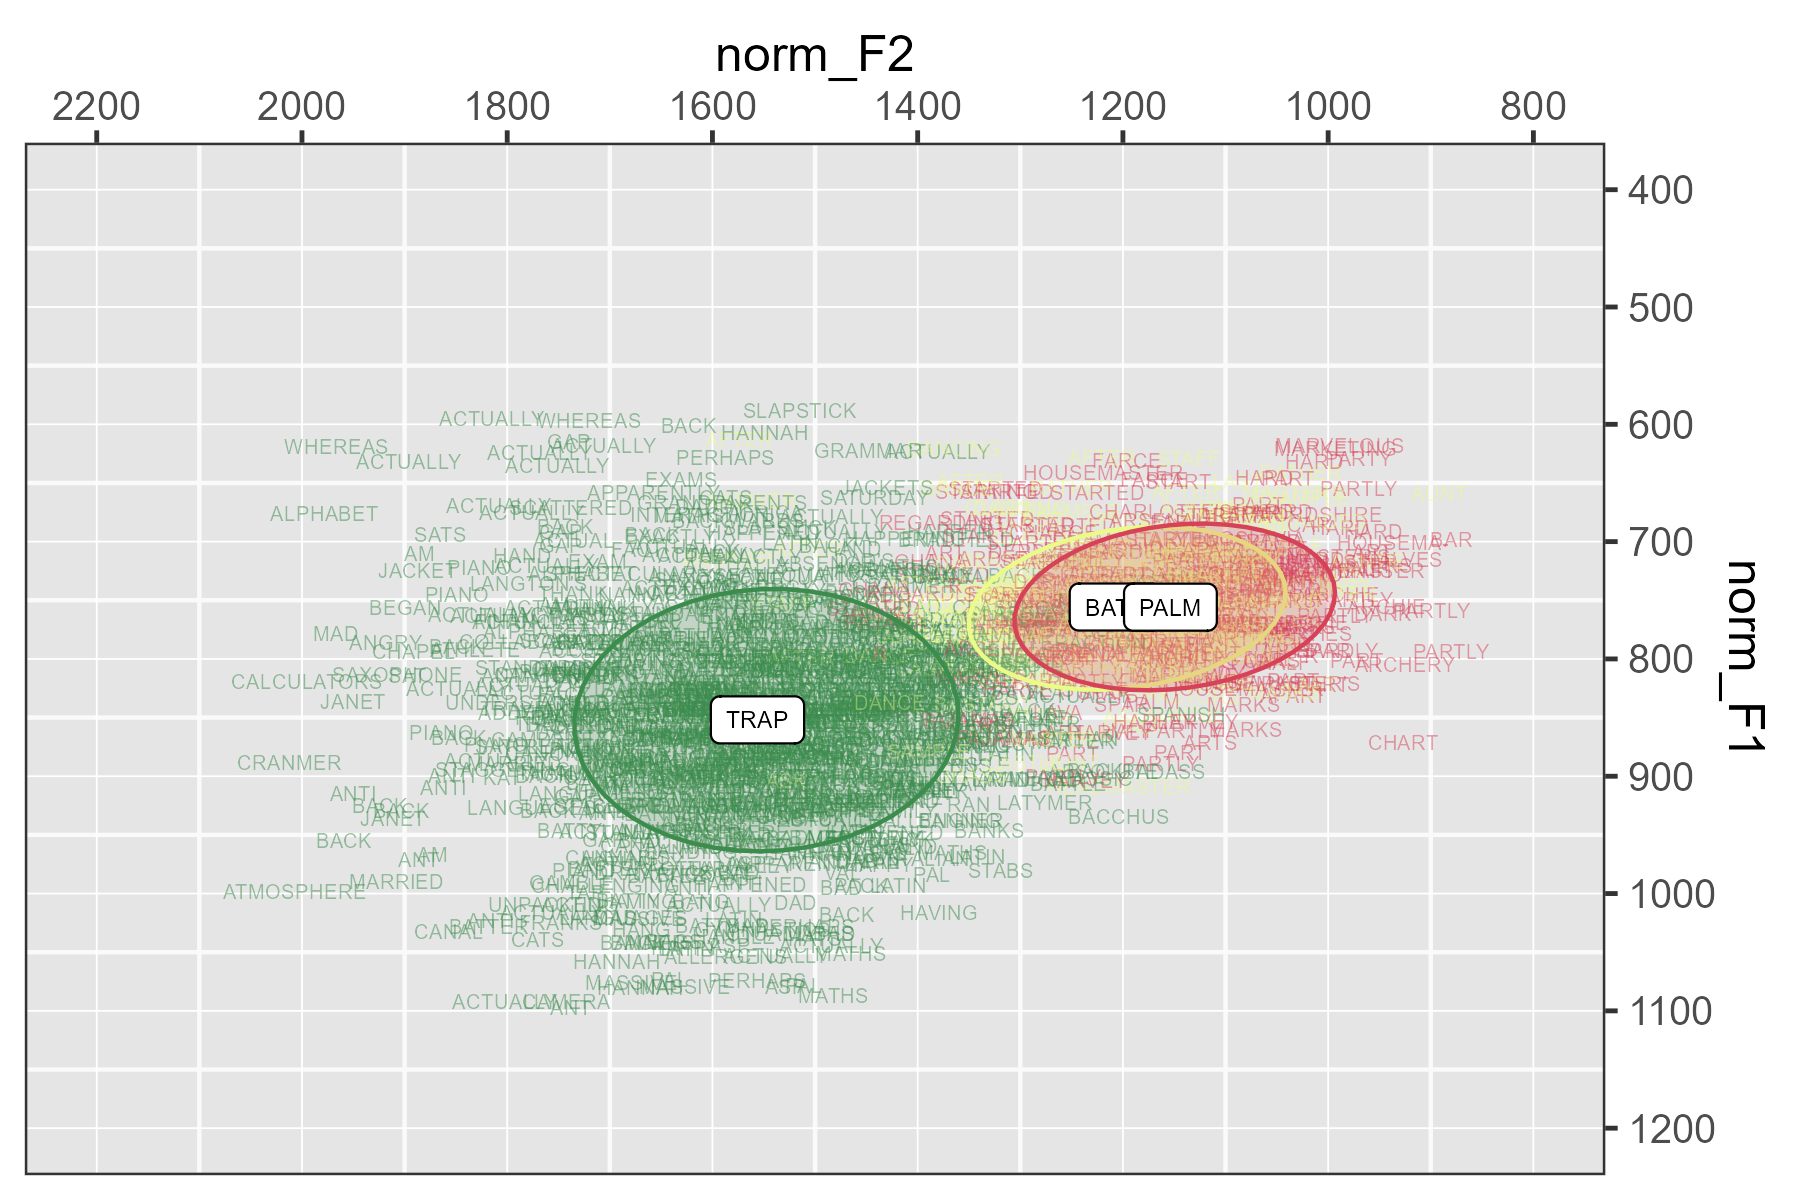
\includegraphics[width=\textwidth]{../figures/TBP-SE-vplot.png}
	\caption{Vowel Space plot of \trap{},\bath{} and \palm{} in the CoRP-SE speakers} \label{fig:TBPvplotSE}
\end{figure}


\subsubsection{F1 of the CoRP-SE speakers}
The best fit model of F1 of \trap{}, \bath{}, and \palm{} in the CoRP-SE speakers is shown in table \ref{tbl:TBPF1SE}, which includes an interaction effect of lexical set and speaker sex. The calculation of the interaction can be seen in table \ref{tbl:TBPF1SE-inter} (note, the cells in grey are marked to show that none of the effects that distinguish the \palm{} values from the \bath{} values had a t-value greater than 1.4 so could be considered negligible). This demonstrates that \bath{} patterns with \palm{} and the \TB{} split in the South East speakers has an overall higher vowel in \trap{} than in \bath{} (see figure \ref{fig:TBPF1SE}). A mean F1 difference of +98Hz (calculated between \bath{} and \trap{}, excluding the \palm{} effect). This is larger in female speakers (+117Hz) due to a lower \bath{} and higher \trap{}, and lower in the male speakers (+79Hz) due to a higher \bath{} and lower \trap{}. Overral the mean F1 for vowels in \bath{} words is 740Hz, for \palm{} words 755Hz, and for \trap{} words 857Hz.
% latex table generated in R 4.1.0 by xtable 1.8-4 package
% Wed Jan 12 09:40:55 2022
\begin{table}[ht]
\centering
\begin{tabular}{lrr}
  \hline
fixedeffect & estimate & tvalue \\ 
  \hline
(Intercept) & 739.50 & 61.88 \\ 
  lexSetPALM & 15.90 & 1.40 \\ 
  lexSetTRAP & 117.49 & 12.25 \\ 
  sexMale & 13.94 & 0.81 \\ 
  ageGroupSum1 & -0.60 & -0.09 \\ 
  freq.zipf\_z & 0.44 & 0.14 \\ 
  styleminimalpair & 42.22 & 2.04 \\ 
  stylewordlist & 32.41 & 3.38 \\ 
  has\_codaSum1 & 2.42 & 0.71 \\ 
  lexSetPALM:sexMale & -9.63 & -0.61 \\ 
  lexSetTRAP:sexMale & -38.95 & -2.93 \\ 
   \hline
\end{tabular}
\caption{Linear Mixed Effects Model of F1 of \textsc{trap},\textsc{bath}, and \textsc{palm} in CoRP-SE speakers \label{tbl:TBPF1SE}} 
\end{table}


% Table generated by Excel2LaTeX from sheet 'TBPF1SE'
\begin{table}[htbp]
	\centering
	\begin{tabular}{lrrrr}
		\hline
		& \multicolumn{1}{l}{\bath{}} & \multicolumn{1}{l}{\palm{}} & \multicolumn{1}{l}{\trap{}} & \multicolumn{1}{l}{\TB{} difference} \\
		\hline
		Female & 764.37 & \cellcolor[rgb]{ .816,  .808,  .808} 780.27 & 881.86 & 117.49 \\
		Male  & 778.31 & \cellcolor[rgb]{ .816,  .808,  .808} 784.58 & 856.85 & 78.54 \\
		Mean  & 771.34 & \cellcolor[rgb]{ .816,  .808,  .808} 782.43 & 869.36 & 98.02 \\
		\hline
	\end{tabular}
	\caption{Interactions effects of lexical set and speaker sex on F1 of \trap{}, \bath{}, and \palm{} in CoRP-SE speakers (calculated from interactions in table \ref{tbl:TBPF1SE})}
	\label{tbl:TBPF1SE-inter}
\end{table}

\begin{figure}[h]
	\includesvg[width=\textwidth]{../figures/TBP-SE-F1.svg}
	\caption{F1 of \bath{}, \palm{}, and \trap{}  in CoRP-SE speakers} \label{fig:TBPF1SE}
\end{figure}

\subsubsection{F2 of the CoRP-SE speakers}
The best fit model for the F2 of \trap{}, \bath{}, and \palm{}, can be seen in table \ref{tbl:TBPF2SE}. Similar to the model of F1 there is a difference between \bath{} and \trap{} (+363Hz, t=18.97) but little to none between \bath{} and \palm{} (-39Hz, t = -1.81), again supporting past evidence that \bath{} patterns with \palm{} in the South East, this difference is shown in figure \ref{fig:TBPF2SE}. The mean F2 for vowels in the \bath{} lexical set is 1215Hz, for \palm{} 1175Hz, and for \trap{} 1578Hz; there is no other significant variation.

% latex table generated in R 4.1.0 by xtable 1.8-4 package
% Mon Dec 13 17:20:45 2021
\begin{table}[ht]
\centering
\begin{tabular}{lrr}
  \hline
fixedeffect & estimate & tvalue \\ 
  \hline
(Intercept) & 1214.63 & 46.57 \\ 
  lexSetPALM & -39.41 & -1.81 \\ 
  lexSetTRAP & 363.19 & 18.97 \\ 
  sexSum1 & 1.80 & 0.13 \\ 
  ageGroupSum1 & 25.92 & 1.85 \\ 
  freq.zipf\_z & 3.80 & 0.59 \\ 
  styleSum1 & -25.27 & -1.59 \\ 
  styleSum2 & 23.53 & 0.90 \\ 
  has\_codaSum1 & -1.73 & -0.25 \\ 
  time\_z & -6.25 & -1.46 \\ 
   \hline
\end{tabular}
\caption{Linear Mixed Effects Model of F2 of \textsc{trap},\textsc{bath}, and \textsc{palm} in CoRP-SE speakers \label{tbl:TBPF2SE}} 
\end{table}


\begin{figure}[h]
	\includesvg[width=\textwidth]{../figures/TBP-SE-F2.svg}
	\caption{F2 of \bath{}, \palm{}, and \trap{}  in CoRP-SE speakers} \label{fig:TBPF2SE}
\end{figure}


\subsubsection{Duration of the CoRP-SE speakers}

%% latex table generated in R 4.1.0 by xtable 1.8-4 package
% Wed Jan 19 10:34:36 2022
\begin{table}[ht]
\centering
\begin{tabular}{lrr}
  \hline
fixedeffect & estimate & tvalue \\ 
  \hline
(Intercept) & 120.55 & 15.50 \\ 
  lexSetPALM & 13.26 & 1.40 \\ 
  lexSetTRAP & -23.40 & -2.91 \\ 
  styleminimalpair & 33.40 & 0.97 \\ 
  stylewordlist & 66.20 & 5.22 \\ 
  sexSum1 & 7.81 & 2.82 \\ 
  ageGroupSum1 & 1.02 & 0.38 \\ 
  freq.zipf\_z & 0.30 & 0.12 \\ 
  has\_codaSum1 & -8.74 & -3.27 \\ 
  time\_z & 6.01 & 3.33 \\ 
  folVcSum1 & 3.04 & 1.12 \\ 
  lexSetPALM:styleminimalpair & 28.80 & 0.65 \\ 
  lexSetTRAP:styleminimalpair & -12.71 & -0.30 \\ 
  lexSetPALM:stylewordlist & 57.38 & 2.77 \\ 
  lexSetTRAP:stylewordlist & -14.71 & -0.92 \\ 
   \hline
\end{tabular}
\caption{Linear Mixed Effects Model of duration of \textsc{trap},\textsc{bath}, and \textsc{palm} in CoRP-SE speakers \label{tbl:TBPdurSE}} 
\end{table}

% latex table generated in R 4.1.0 by xtable 1.8-4 package
% Mon Feb 07 14:43:34 2022
\begin{table}[ht]
\centering
\begin{tabular}{lrr}
  \hline
fixedeffect & estimate & tvalue \\ 
  \hline
(Intercept) & 2.09 & 30.02 \\ 
  lexSetPALM & 0.06 & 0.78 \\ 
  lexSetTRAP & -0.12 & -2.08 \\ 
  has\_codaTRUE & 0.03 & 0.44 \\ 
  sexSum1 & 0.02 & 2.48 \\ 
  ageGroupSum1 & 0.00 & 0.33 \\ 
  freq.zipf\_z & -0.00 & -0.03 \\ 
  styleSum1 & -0.05 & -1.19 \\ 
  styleSum2 & -0.04 & -0.47 \\ 
  time\_z & 0.04 & 1.93 \\ 
  folVcSum1 & 0.01 & 0.82 \\ 
  lexSetPALM:has\_codaTRUE & -0.01 & -0.15 \\ 
  lexSetTRAP:has\_codaTRUE & 0.05 & 0.74 \\ 
  styleSum1:time\_z & -0.03 & -1.36 \\ 
  styleSum2:time\_z & 0.02 & 0.52 \\ 
   \hline
\end{tabular}
\caption{Linear Mixed Effects Model of log10(duration) of \textsc{trap},\textsc{bath}, and \textsc{palm} in CoRP-SE speakers \label{tbl:TBPlogdurSE}} 
\end{table}

The model for duration of the \trap{}, \bath{}, and \palm{} vowels is shown in table \ref{tbl:TBPdurSE}. The best fit model included an interaction between lexical set and presence of coda, as shown in table \ref{tbl:TBPdurSE-inter}. The mean duration of the vowel in the \bath{} words is 123msec However, the only significant effect seen is that of \trap{}, which is 28msec shorter than \palm{} and \bath{}. This shows that \bath{} words are broadly the same length as \palm{} words and different to \trap{} words, demonstrating that the \TB{} split is also found in duration.

% Table generated by Excel2LaTeX from sheet 'TBPlogdurSE'
\begin{table}[htbp]
	\centering
	\begin{tabular}{lrrrrrr}
		& \multicolumn{1}{l}{\bath{}} & \multicolumn{1}{l}{\palm{}} & \multicolumn{1}{l}{\trap{}} & \multicolumn{1}{l}{\trap{}-bath{} difference} & \multicolumn{1}{l}{\palm{}-\bath{} difference} & \multicolumn{1}{l}{\trap{}-\palm{} difference} \\
		\hline
		has\_codaFALSE & 123.0269 & 141.2538 & 95.49926 & -27.53 & 18.23 & -45.75 \\
		has\_codaTRUE & 131.8257 & 147.9108 & 114.8154 & -17.01 & 16.09 & -33.10 \\
		\hline
		average & 127.4263 & 144.5823 & 105.1573 & -22.27 & 17.16 & -39.42 \\
		\hline
	\end{tabular}%s
	\caption{Interaction effects of lexical set and presence of coda on \trap{}, \bath{}, and \palm{} in CoRP-SE speakers (converted to msec)} 
	\label{tbl:TBPdurSE-inter}%
\end{table}%





\todocontentinline{Without perception data it is difficult to tell if this length difference is contributing to the status of the \bath{} words.}



\begin{figure}[h]
	\includesvg[width=\textwidth]{../figures/TBP-SE-dur-all.svg}
	\caption{Duration of \bath{}, \palm{}, and \trap{}  in CoRP-SE speakers} \label{fig:TBPdurSE}
\end{figure}


\subsection{The Split in DECTE speakers}
In models of F1, F2, and duration, the DECTE speakers do not show any difference between \trap{} and \bath{} words. The difference between \trap{} and \palm{} is 70Hz in F1 and 205Hz in F2. These speakers show a more spread out \palm{} distribution than the CoRP-SE speakers but they show no difference between \trap{} and \bath{}; there is no evidence of a \TB{} split, the models demonstrating this can be seen below.

\begin{figure}[h]
	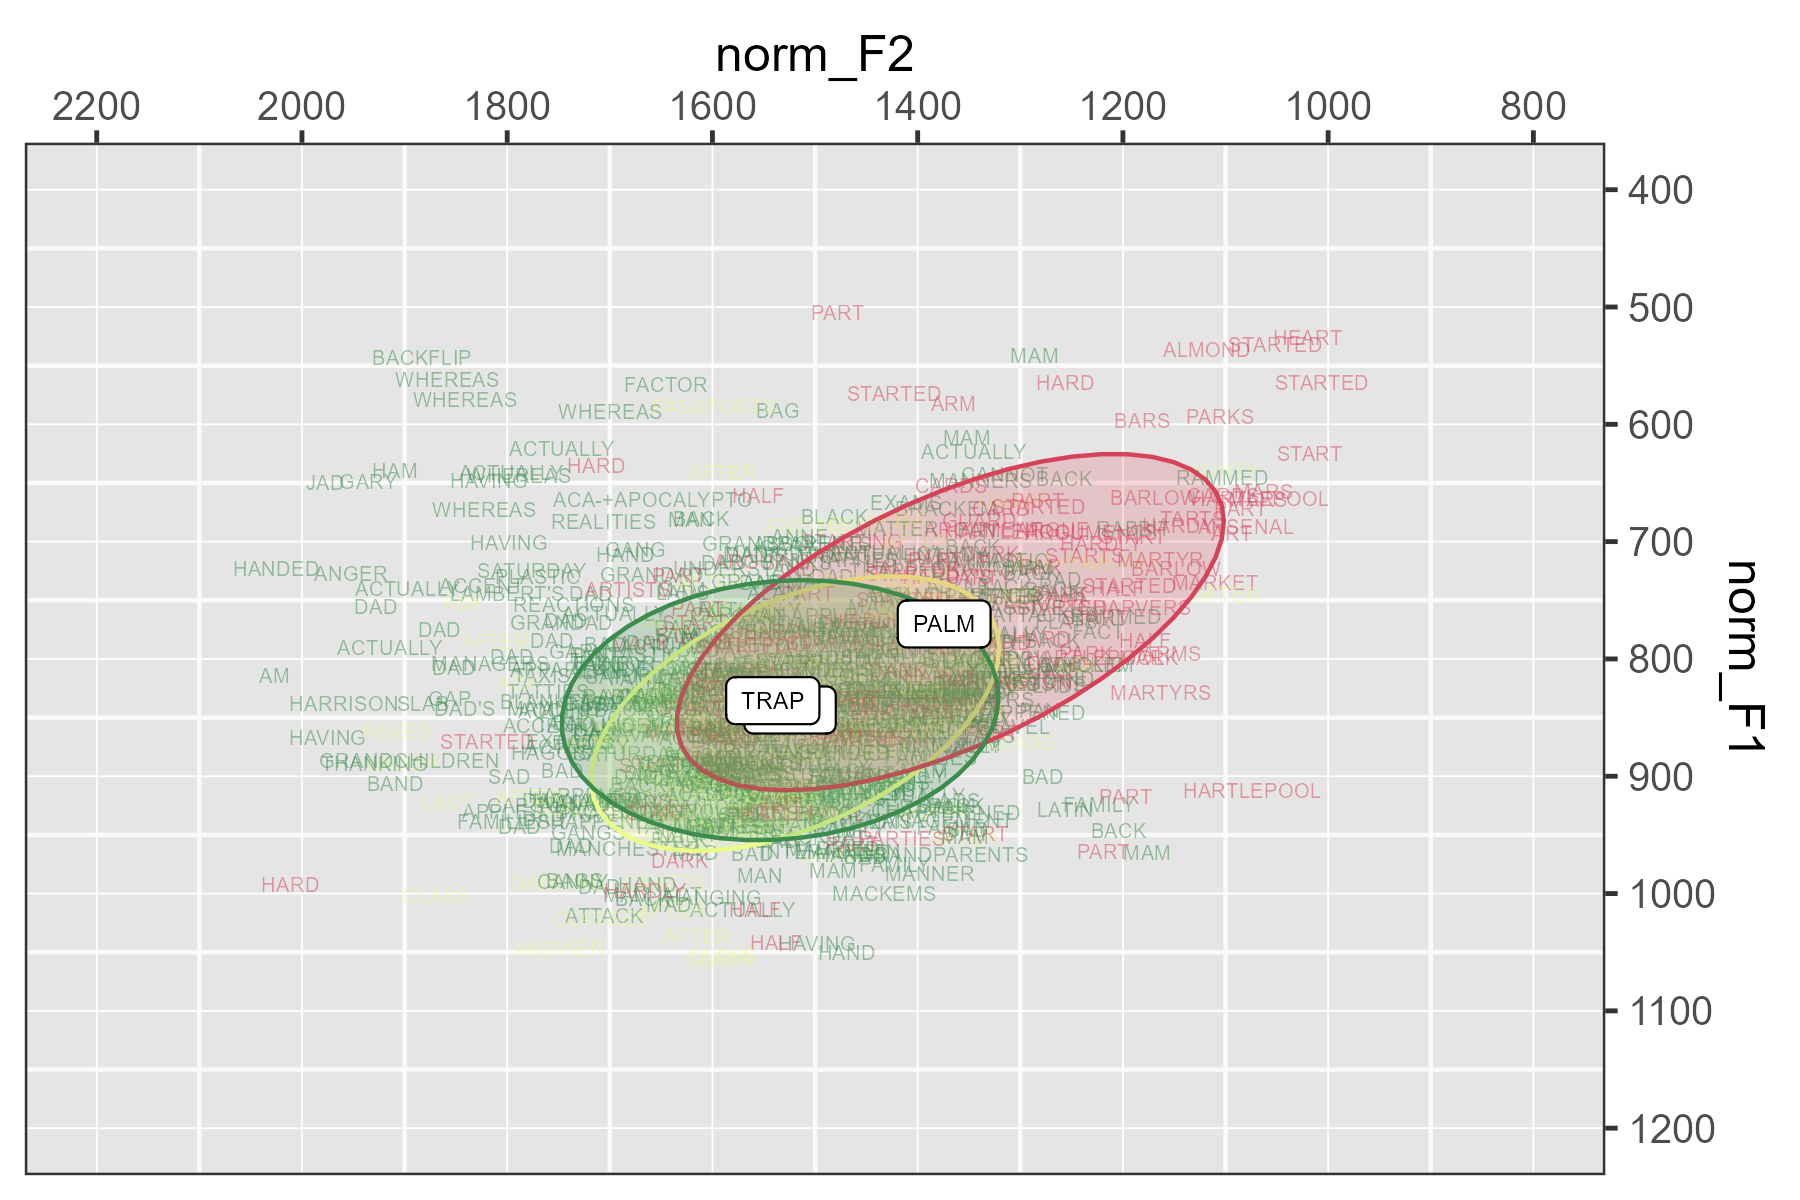
\includegraphics[width=\textwidth]{../figures/TBP-DE-vplot.png}
	\caption{Vowel Space plot of \trap{},\bath{} and \palm{} in the DECTE speakers} \label{fig:TBPvplotDE}
\end{figure}



\subsubsection{F1 of the DECTE speakers}
% latex table generated in R 4.1.0 by xtable 1.8-4 package
% Wed Dec 08 10:21:28 2021
\begin{table}[ht]
\centering
\begin{tabular}{lrr}
  \hline
fixedeffect & estimate & tvalue \\ 
  \hline
(Intercept) & 841.89 & 65.90 \\ 
  lexSetPALM & -70.43 & -4.26 \\ 
  lexSetTRAP & -0.90 & -0.07 \\ 
  sexMale & -45.42 & -2.39 \\ 
  ageGroupSum1 & 23.54 & 6.07 \\ 
  freq.zipf\_z & 8.10 & 1.69 \\ 
  has\_codaSum1 & 2.41 & 0.48 \\ 
  time\_z & -4.42 & -0.85 \\ 
  lexSetPALM:sexMale & -9.28 & -0.35 \\ 
  lexSetTRAP:sexMale & -1.91 & -0.09 \\ 
   \hline
\end{tabular}
\caption{Linear Mixed Effects Model of F1 of \textsc{trap},\textsc{bath}, and \textsc{palm} in DECTE-NE speakers \label{tbl:TBPF1DE}} 
\end{table}

Table \ref{tbl:TBPF1DE} shows the best fit model for F1 of the \trap{}, \bath{}, and \palm{} words in the DECTE speakers. The mean F2 of the vowel in the \bath{} words is shown to be 842Hz, 70Hz higher (lower in the mouth) than the \palm{} words, which have a mean of 771 Hz and almost identical to the \trap{} words (mean = 841Hz). As would be expected from speakers in the North of England, the DECTE speakers are not showing an evidence of a \TB{} split in F1.

\begin{figure}[h]
	\includesvg[width=\textwidth]{../figures/TBP-DE-F1.svg}
	\caption{F1 of \trap{}, \bath{} and \palm{}  in DECTE speakers} \label{fig:TBF1DE}
\end{figure}

\subsubsection{F2 of the DECTE speakers}
The best fit model for the F2 of the \trap{}, \bath{}, and \palm{} words is shown in table \ref{tbl:TBPF2DE}. The vowels in the \bath{} words have a mean of 1505Hz and  in \palm{} words, 1324 Hz (difference of 181Hz), showing that \bath{} is further forward in the vowel space. This is supported by the negligible difference between the \bath{} and \trap{} words, which have a mean of 1530 Hz. The difference between \palm{} and \trap{}/\bath{} is also smaller than in CoRP-SE speakers. 

% latex table generated in R 4.1.0 by xtable 1.8-4 package
% Wed Dec 08 11:21:55 2021
\begin{table}[ht]
\centering
\begin{tabular}{lrr}
  \hline
fixedeffect & estimate & tvalue \\ 
  \hline
(Intercept) & 1504.91 & 37.87 \\ 
  lexSetPALM & -180.69 & -6.42 \\ 
  lexSetTRAP & 24.61 & 1.06 \\ 
  sexSum1 & 36.40 & 1.12 \\ 
  ageGroupSum1 & -17.55 & -0.53 \\ 
  freq.zipf\_z & 0.74 & 0.08 \\ 
  has\_codaSum1 & -5.21 & -0.57 \\ 
  time\_z & -18.10 & -1.99 \\ 
   \hline
\end{tabular}
\caption{Linear Mixed Effects Model of F2 of \textsc{trap},\textsc{bath}, and \textsc{palm} in DECTE-NE speakers \label{tbl:TBPF2DE}} 
\end{table}


\begin{figure}[h]
	\includesvg[width=\textwidth]{../figures/TBP-DE-F2.svg}
	\caption{F2 of \trap{}, \bath{} and \palm{}  in DECTE speakers} \label{fig:TBF2DE}
\end{figure}


\subsubsection{Duration of the DECTE speakers}
% latex table generated in R 4.1.0 by xtable 1.8-4 package
% Mon Feb 07 17:22:21 2022
\begin{table}[ht]
\centering
\begin{tabular}{lrr}
  \hline
fixedeffect & estimate & tvalue \\ 
  \hline
(Intercept) & 1.99 & 33.16 \\ 
  lexSetPALM & -0.04 & -0.40 \\ 
  lexSetTRAP & -0.11 & -1.86 \\ 
  has\_codaTRUE & -0.03 & -0.46 \\ 
  sexSum1 & 0.00 & 0.06 \\ 
  ageGroupSum1 & -0.01 & -0.87 \\ 
  freq.zipf\_z & -0.00 & -0.21 \\ 
  time\_z & -0.00 & -0.16 \\ 
  folVcSum1 & 0.01 & 0.44 \\ 
  lexSetPALM:has\_codaTRUE & 0.14 & 1.26 \\ 
  lexSetTRAP:has\_codaTRUE & 0.09 & 1.33 \\ 
   \hline
\end{tabular}
\caption{Linear Mixed Effects Model of duration of \textsc{trap},\textsc{bath}, and \textsc{palm} in DECTE-NE speakers \label{tbl:TBPdurDE}} 
\end{table}

The best fit model of duration in the DECTE speakers can be seen in table \ref{tbl:TBPdurDE} and the interaction calculation (converted to msec) is shown in table \ref{tbl:TBPdurDE-inter}. The model shows that the mean vowel length in the \bath{} words is 94msec long. Those with a coda are approximately the same length as the \trap{} words with codas (4Hz difference), though in the words without codas the difference is larger (-22msec). There is a difference between \trap{} and \palm{} (-20msec), however, all of these values are closer to the value for the \trap{} words in the CoRP-SE speakers than to the \palm{} and \bath{} values in the CoRP-SE speakers demonstrating that not only do the DECTE speakers not show a \TB{} split in duration, they also broadly do not have a long \palm{} vowel. This supports the conclusion drawn from the variation found in F2 that the \palm{} vowel is not consistently the same in DECTE speakers as in the CoRP-SE speakers.

\todocontent{say more about the interaction and codas?}

% Table generated by Excel2LaTeX from sheet 'TBPlogdurDE'
\begin{table}[htbp]
	\centering

	\begin{tabular}{lrrrrrr}
		& \multicolumn{1}{l}{\bath{}} & \multicolumn{1}{l}{\palm{}} & \multicolumn{1}{l}{\trap{}} & \multicolumn{1}{l}{\TB{} diff} & \multicolumn{1}{l}{\palm{}-\bath{} diff} & \multicolumn{1}{l}{\trap{}-\palm{} diff} \\
		no coda & 97.72372 & 89.12509 & 75.85776 & -21.87 & -8.60 & -13.27 \\
		coda & 91.20108 & 114.8154 & 87.09636 & -4.10 & 23.61 & -27.72 \\
		mean  & 94.4624 & 101.9702 & 81.47706 & -12.99 & 7.51  & -20.49 \\
	\end{tabular}%
		\caption{Interaction effects of lexical set and presence of coda on \trap{}, \bath{}, and \palm{} in DECTE speakers} \label{tbl:TBPdurDE-inter}%
\end{table}%


\begin{figure}[h]
	\includesvg[width=\textwidth]{../figures/TBP-DE-dur-all.svg}
	\caption{Duration of \trap{}, \bath{} and \palm{}  in DECTE speakers} \label{fig:TBdurDE}
\end{figure}

\subsection{The Split in CoRP-NE speakers}
The CoRP-NE speakers show little to no difference in F1 or F2 that could be evidence for a \TB{} split (though F2 is a little more complex, details below). The difference between \trap{} and \palm{} in F1 is 86Hz and in F2 is 329Hz.

\begin{figure}[h]
	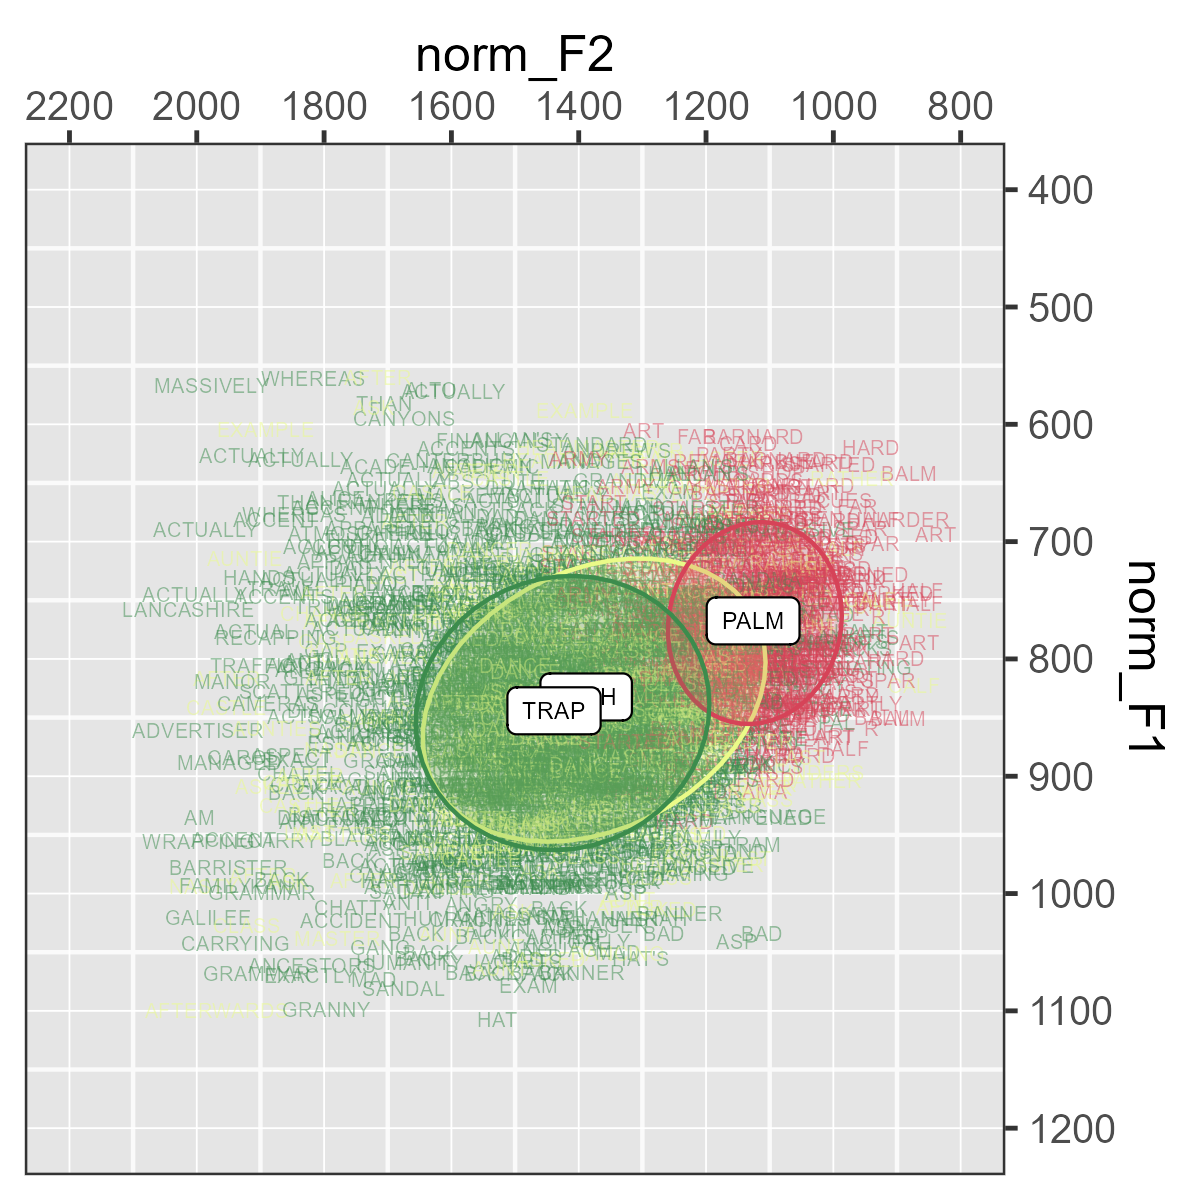
\includegraphics[width=\textwidth]{../figures/TBP-NE-vplot.png}
	\caption{Vowel Space plot of \trap{},\bath{} and \palm{} in the CoRP-NE speakers} \label{fig:TBPvplotNE}
\end{figure}



\subsubsection{F1 of the CoRP-NE speakers}
Table \ref{tbl:TBPF1NE} shows the best fit model for the CoRP-NE speakers. There is a three way interaction between lexical set, speaker sex, and speaker age group, which is summarised in table \ref{TBPF1NE-inter}. This table shows that the largest \TB{} difference is found in the Old Male group (which is only one speaker, who has spent more time in the south of England than other speakers)

% latex table generated in R 4.1.0 by xtable 1.8-4 package
% Mon Dec 20 15:31:02 2021
\begin{table}[ht]
\centering
\begin{tabular}{lrr}
  \hline
fixedeffect & estimate & tvalue \\ 
  \hline
(Intercept) & 814.30 & 43.81 \\ 
  lexSetPALM & -52.55 & -2.88 \\ 
  lexSetTRAP & 78.88 & 4.97 \\ 
  sexMale & 10.88 & 0.40 \\ 
  ageGroupYoung & 45.78 & 2.41 \\ 
  freq.zipf\_z & 1.58 & 0.53 \\ 
  styleSum1 & -16.23 & -2.16 \\ 
  styleSum2 & -4.94 & -0.39 \\ 
  has\_codaSum1 & 1.69 & 0.52 \\ 
  time\_z & 1.50 & 0.64 \\ 
  lexSetPALM:sexMale & 15.55 & 0.55 \\ 
  lexSetTRAP:sexMale & -55.72 & -2.34 \\ 
  lexSetPALM:ageGroupYoung & -9.22 & -0.48 \\ 
  lexSetTRAP:ageGroupYoung & -74.15 & -4.47 \\ 
  sexMale:ageGroupYoung & -33.80 & -1.10 \\ 
  lexSetPALM:sexMale:ageGroupYoung & -30.44 & -0.98 \\ 
  lexSetTRAP:sexMale:ageGroupYoung & 59.93 & 2.25 \\ 
   \hline
\end{tabular}
\caption{Linear Mixed Effects Model of F1 of \textsc{trap},\textsc{bath}, and \textsc{palm} in CoRP-NE speakers \label{tbl:TBPF1NE}} 
\end{table}


% Table generated by Excel2LaTeX from sheet 'TBPF1NE'
\begin{table}[htbp]
	\centering
	\begin{tabular}{lrrrrrr}
		\hline
		& \multicolumn{1}{l}{\bath{}} & \multicolumn{1}{l}{\palm{}} & \multicolumn{1}{l}{\trap{}} & \multicolumn{1}{l}{\TB{} diff} & \multicolumn{1}{l}{\palm{}-\bath{} diff} & \multicolumn{1}{l}{\trap{}-\palm{} diff} \\
		\hline
		Old Female & 814.30 & 761.75 & 893.18 & 78.88 & -52.55 & 131.43 \\
		Old Male & 825.18 & 788.18 & 848.34 & 23.16 & -37.00 & 60.16 \\
		Young Female & 860.08 & 798.31 & 864.81 & 4.73  & -61.77 & 66.50 \\
		Young Male & 837.16 & 760.50 & 846.10 & 8.94  & -76.66 & 85.60 \\
		Mean  & 834.18 & 777.19 & 863.11 & 28.93 & -57.00 & 85.92 \\
		\hline
	\end{tabular}%
	\caption{Interaction effects of lexical set, speaker sex and speaker age group on F1 of \trap{}, \bath{}, and \palm{} in CoRP-NE speakers (calculated from interactions in table \ref{tbl:TBPF1NE})} \label{TBPF1NE-inter}%
\end{table}%



\begin{figure}[h]
	\includesvg[width=\textwidth]{../figures/TBP-NE-F1.svg}
	\caption{F1 of \trap{}, \bath{} and \palm{} in DECTE speakers} \label{fig:TF1NE}
\end{figure}

\subsubsection{F2 of the CoRP-NE speakers}
Table \ref{tbl:TBPF2NE}  shows the best fit model for F2 of the CoRP-NE speakers; the model included a three way interaction between lexical set, speaker sex, and speaker age group, the results of which are shown in table \ref{tbl:TBPF2NEinter}. Despite the interaction effects, it can be seen that the majority of speakers show a very small \TB{} difference (mean = 90Hz). The largest \TB{} difference (and smallest \palm{}-\bath{} difference) is seen in the old male group, which is only one speaker, who has spent more time in the south than the other speakers.
The F2 values could be interpreted as a \bath{} target that is slightly further back than \trap{}, however, it is also possible that the difference is due to some individual \bath{} words having a \palm{} target. Further analysis on the \bath{} vowel will be presented below.
% latex table generated in R 4.1.0 by xtable 1.8-4 package
% Wed Dec 15 15:10:03 2021
\begin{table}[ht]
\centering
\begin{tabular}{lrr}
  \hline
fixedeffect & estimate & tvalue \\ 
  \hline
(Intercept) & 1334.28 & 29.30 \\ 
  lexSetPALM & -214.93 & -5.86 \\ 
  lexSetTRAP & 80.85 & 2.52 \\ 
  sexMale & 5.92 & 0.08 \\ 
  ageGroupYoung & 45.92 & 0.92 \\ 
  has\_codaSum1 & 5.25 & 0.73 \\ 
  freq.zipf\_z & -1.75 & -0.26 \\ 
  time\_z & -2.45 & -0.58 \\ 
  lexSetPALM:sexMale & 24.34 & 0.46 \\ 
  lexSetTRAP:sexMale & 106.53 & 2.36 \\ 
  lexSetPALM:ageGroupYoung & -28.76 & -0.79 \\ 
  lexSetTRAP:ageGroupYoung & -26.68 & -0.84 \\ 
  sexMale:ageGroupYoung & 39.27 & 0.46 \\ 
  lexSetPALM:sexMale:ageGroupYoung & -89.44 & -1.52 \\ 
  lexSetTRAP:sexMale:ageGroupYoung & -124.64 & -2.48 \\ 
   \hline
\end{tabular}
\caption{Linear Mixed Effects Model of F2 of \textsc{trap},\textsc{bath}, and \textsc{palm} in CoRP-NE speakers \label{tbl:TBPF2NE}} 
\end{table}

% Table generated by Excel2LaTeX from sheet 'TBPF2NE'
\begin{table}[htbp]
	\centering
	\begin{tabular}{lrrrrr}
		\hline
		& \multicolumn{1}{l}{\bath{}} & \multicolumn{1}{l}{\palm{}} & \multicolumn{1}{l}{\trap{}} & \multicolumn{1}{l}{\TB{} difference} & \multicolumn{1}{l}{\palm{}-\bath{} difference} \\
		\hline
		Old Female & 1334.28 & 1119.35 & 1415.13 & 80.85 & -214.93 \\
		Old Male & 1343.20 & 1152.61 & 1530.58 & 187.38 & -190.59 \\
		Young Female & 1380.20 & 1136.51 & 1434.37 & 54.17 & -243.69 \\
		Young Male & 1428.39 & 1119.60 & 1464.45 & 36.06 & -308.79 \\
		Mean  & 1371.52 & 1132.02 & 1461.13 & 89.61 & -239.50 \\
		\hline
	\end{tabular}%
	\caption{Interaction effects of lexical set, speaker sex and speaker age group on F2 of \trap{}, \bath{}, and \palm{} in CoRP-NE speakers (calculated from interactions in table \ref{tbl:TBPF2NE})}
	\label{tbl:TBPF2NEinter}%
\end{table}%



\subsubsection{Duration of the CoRP-NE speakers}
Table \ref{tbl:TBPF2NE} shows the best fit model for duration in the CoRP-NE speakers. An interaction effect is seen between lexical set and presence of a coda. This interaction is summarised in table \ref{TBP-NE-dur-mod-inter}. \scs{Trap} and \palm{} are on average 62 msec  apart, and the \palm{} length is closer to the length found in the CoRP-SE speakers, implying that CoRP-NE speaker do not have the shorter \palm{} vowel found in the DECTE speakers. There is a \TB difference present in the words with a coda (-20msec) but none in words without a coda. The difference is less than the difference between \trap{}-\palm{}, and while the mean duration  of the \bath{} (136msec) words is longer than the \trap{} words (126msec) it is not as long as the \palm{} words (189msec). In a form similar to the F2 results above, the duration of the \bath{} values could be interpreted as a target that is slightly further back than \trap{}, or as some individual \bath{} words having a \palm{} target and so pulling the mean duration higher.






% latex table generated in R 4.1.0 by xtable 1.8-4 package
% Tue Feb 08 12:55:56 2022
\begin{table}[ht]
\centering
\begin{tabular}{lrr}
  \hline
fixedeffect & estimate & tvalue \\ 
  \hline
(Intercept) & 2.14 & 35.52 \\ 
  lexSetPALM & 0.16 & 1.49 \\ 
  lexSetTRAP & -0.07 & -1.25 \\ 
  has\_codaTRUE & -0.01 & -0.22 \\ 
  sexSum1 & 0.02 & 1.68 \\ 
  ageGroupSum1 & 0.00 & 0.28 \\ 
  freq.zipf\_z & 0.01 & 1.27 \\ 
  styleSum1 & -0.11 & -5.35 \\ 
  styleSum2 & 0.06 & 1.74 \\ 
  time\_z & 0.00 & 0.38 \\ 
  folVcSum1 & -0.01 & -0.85 \\ 
  lexSetPALM:has\_codaTRUE & -0.04 & -0.34 \\ 
  lexSetTRAP:has\_codaTRUE & 0.07 & 1.14 \\ 
   \hline
\end{tabular}
\caption{Linear Mixed Effects Model of duration of \textsc{trap},\textsc{bath}, and \textsc{palm} in CoRP-NE speakers \label{tbl:TBPdurNE}} 
\end{table}


% Table generated by Excel2LaTeX from sheet 'TBPlogdurSE'
\begin{table}[htbp]
	\centering
	\begin{tabular}{lrrrrrr}
		\hline
		& \multicolumn{1}{l}{\bath{}} & \multicolumn{1}{l}{\palm{}} & \multicolumn{1}{l}{\trap{}} & \multicolumn{1}{l}{\TB{} diff} & \multicolumn{1}{l}{\palm{}-\bath{} diff} & \multicolumn{1}{l}{\trap{}-\palm{} diff} \\
		\hline
		no coda & 138.0384 & 199.5262 & 117.4898 & -20.55 & 61.49 & -82.04 \\
		coda & 134.8963 & 177.8279 & 134.8963 & 0.00  & 42.93 & -42.93 \\
		mean  & 136.4674 & 188.6771 & 126.193 & -10.27 & 52.21 & -62.48 \\
		\hline
	\end{tabular}%
	\caption{Interaction effects of lexical set and presence of coda on duration of \trap{}, \bath{}, and \palm{} in CoRP-NE speakers.} \label{TBP-NE-dur-mod-inter}%
	
\end{table}%


\begin{figure}[h]
	\includesvg[width=\textwidth]{../figures/TBP-NE-dur.svg}
	\caption{Duration of \trap{}, \bath{} and \palm{} in CoRP-NE speakers} \label{fig:TBdurNE}
\end{figure}



\section{\scs{Bath} vowel alone}

\begin{figure}[h]
	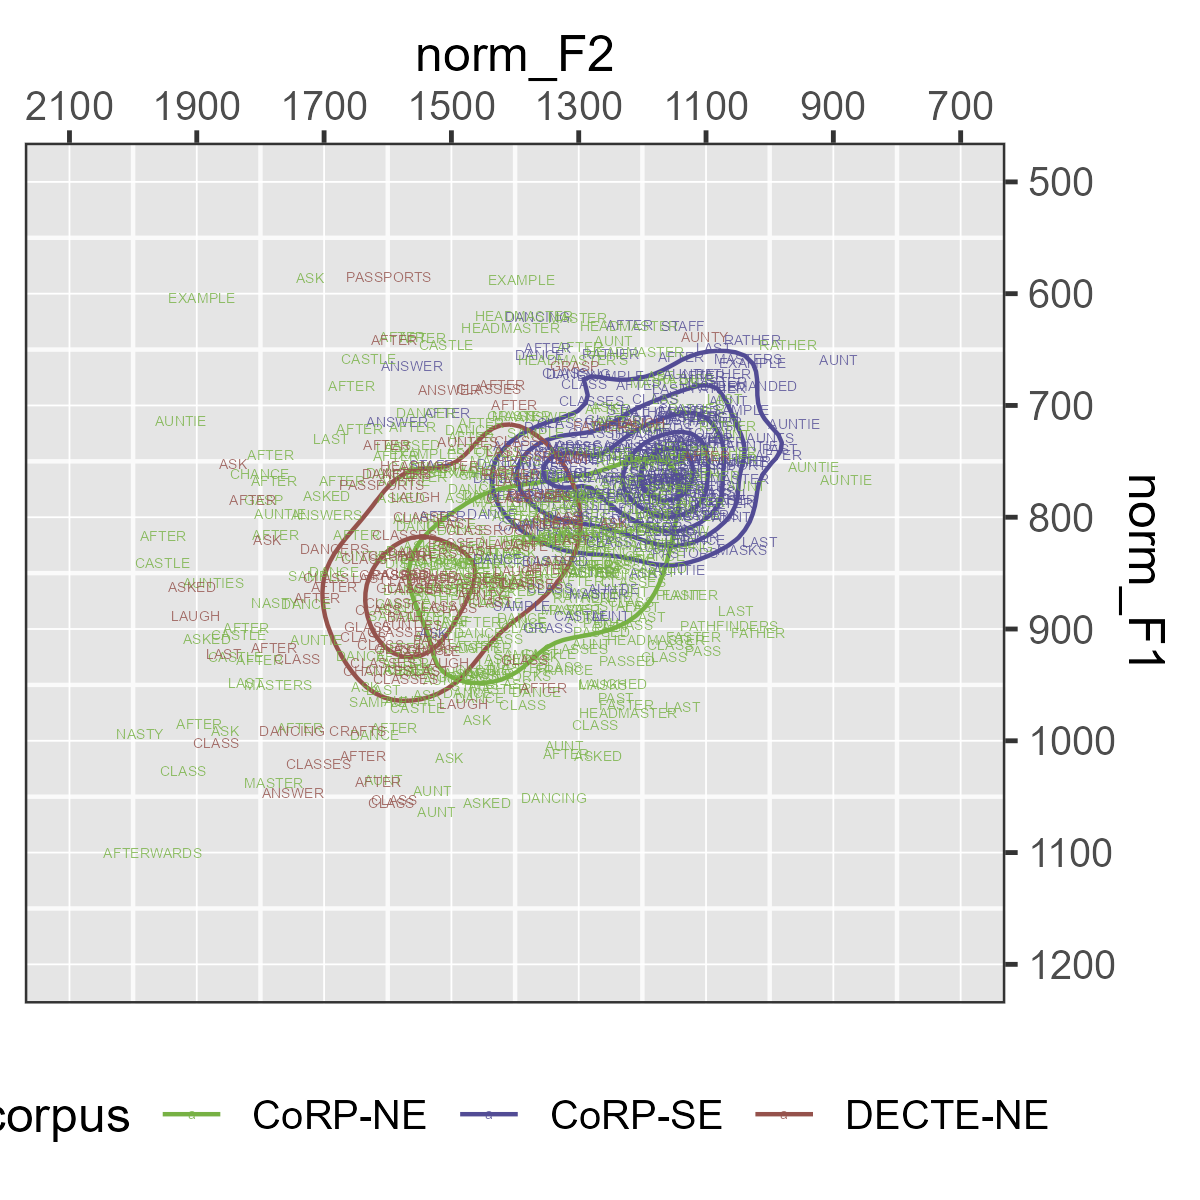
\includegraphics[width=\textwidth]{../figures/B-vplot.png}
	\caption{\bath{}} \label{fig:Bvplot}
\end{figure}



\subsection{F1}
The best fit model of \bath{} in all speaker groups is shown in table \ref{tbl:BF1}. There is a three way interaction between sex, age group and corpus, shown in table \ref{tbl:BF1-inter}. It can be seen that overall the CoRP-NE speakers have a \bath{} vowel at 828Hz, very similar to the height of the DECTE speakers (837Hz), whereas the CoRP-SE speakers have a higher vowel, at 762Hz. While there is variation between male and female, and old and young, none of this variation reaches overlap between the lower vowels (CoRP-NE and DECTE), and the higher vowels (CoRP-SE).

% latex table generated in R 4.1.0 by xtable 1.8-4 package
% Tue Mar 08 11:42:57 2022
\begin{table}[ht]
\centering
\begin{tabular}{lrr}
  \hline
fixedeffect & estimate & tvalue \\ 
  \hline
(Intercept) & 815.06 & 38.48 \\ 
  relevel(corpus, "CoRP-NE")DECTE-NE & 61.18 & 2.53 \\ 
  relevel(corpus, "CoRP-NE")CoRP-SE & -68.19 & -2.82 \\ 
  ageGroupYoung & 40.96 & 1.96 \\ 
  sexMale & 2.08 & 0.07 \\ 
  freq.zipf\_z & 0.78 & 0.12 \\ 
  styleSum1 & -23.64 & -2.19 \\ 
  styleSum2 & 1.15 & 0.06 \\ 
  has\_codaSum1 & -12.15 & -1.69 \\ 
  time\_z & -4.63 & -1.05 \\ 
  relevel(corpus, "CoRP-NE")DECTE-NE:ageGroupYoung & -78.54 & -2.30 \\ 
  relevel(corpus, "CoRP-NE")CoRP-SE:ageGroupYoung & -21.00 & -0.70 \\ 
  relevel(corpus, "CoRP-NE")DECTE-NE:sexMale & -40.70 & -1.05 \\ 
  relevel(corpus, "CoRP-NE")CoRP-SE:sexMale & 19.85 & 0.52 \\ 
  ageGroupYoung:sexMale & -25.99 & -0.78 \\ 
  relevel(corpus, "CoRP-NE")DECTE-NE:ageGroupYoung:sexMale & -8.42 & -0.15 \\ 
  relevel(corpus, "CoRP-NE")CoRP-SE:ageGroupYoung:sexMale & -7.77 & -0.15 \\ 
   \hline
\end{tabular}
\caption{Linear Mixed Effects Model of F1 of \textsc{bath} \label{tbl:BF1}} 
\end{table}





\subsection{F2}
Table \ref{tbl:BF2} shows the best fit model for F2 of the vowel in \bath{} words in all three speaker groups. Modelling the \bath{} words alone shows that the CoRP-NE speakers have a vowel with F2 between the CoRP-SE speakers (-144Hz lower) and DECTE speakers (173Hz higher). From this model it is difficult to tell if this is truly a vowel with a mean in between or the effect of both positions existing with the set of tokens. 

% latex table generated in R 4.1.0 by xtable 1.8-4 package
% Mon Jan 31 13:43:14 2022
\begin{table}[ht]
\centering
\begin{tabular}{lrr}
  \hline
fixedeffect & estimate & tvalue \\ 
  \hline
(Intercept) & 1346.66 & 38.65 \\ 
  relevel(corpus, "CoRP-NE")DECTE-NE & 173.11 & 3.62 \\ 
  relevel(corpus, "CoRP-NE")CoRP-SE & -143.53 & -3.12 \\ 
  sexMale & 40.09 & 0.92 \\ 
  ageGroupSum1 & -5.17 & -0.32 \\ 
  freq.zipf\_z & 26.29 & 1.58 \\ 
  has\_codaSum1 & -24.64 & -1.27 \\ 
  time\_z & -5.45 & -0.72 \\ 
  relevel(corpus, "CoRP-NE")DECTE-NE:sexMale & -148.92 & -2.07 \\ 
  relevel(corpus, "CoRP-NE")CoRP-SE:sexMale & -50.06 & -0.69 \\ 
   \hline
\end{tabular}
\caption{Linear Mixed Effects Model of F2 of \textsc{bath} \label{tbl:BF2}} 
\end{table}


\begin{figure}[h]
	\includesvg[width=\textwidth]{../figures/B-F2.svg}
	\caption{F2 of \bath{}} \label{fig:BF2NE}
\end{figure}




\subsection{Duration}



	
	
	
	
	
	
	\pagebreak
	\bibliography{../../../References/methodology,
		../../../References/rRP
		../../../References/trapBath,
		../../../References/tynesideEnglish
	}
	
	
\end{document} 